\subsection{BeRTOS}
\subsubsection{Licence}
GNU GPL modifiée :
\begin{verbatim}
# As a special exception, you may use this file as part of a free software
# library without restriction.  Specifically, if other files instantiate
# templates or use macros or inline functions from this file, or you compile
# this file and link it with other files to produce an executable, this
# file does not by itself cause the resulting executable to be covered by
# the GNU General Public License.  This exception does not however
# invalidate any other reasons why the executable file might be covered by
# the GNU General Public License.
\end{verbatim}
%C'est dommage mais pas bloquant.

\subsubsection{Code source}
Le code source est disponible à \url{https://github.com/develersrl/bertos}. Il y a
des liens vers bertos.org qui sont tous redirigé vers le projet github donc pas
d'autre site. La documentation à été générée avec doxygen.

\subsubsection{Plateformes cible}
Dans le sous dossier boards il y a 4 cartes à base de STM32 :
\begin{itemize}
	\item nucleo-l152re ;
	\item stm32-p103 ;
	\item stm3220g-eval ;
	\item stm32VLDiscovery.
\end{itemize}

\subsubsection{Communauté}
Le dépôt a été archivé il y a 2 ans après une dizaine d'années d'activité. Il n'y a
donc plus de communauté active ce qui me semble rédhibitoire.

\subsubsection{Acceptabilité}
\begin{tabular}{lll}
\toprule
	Critère				&	Validé		&	Commentaire	\\
\midrule
	Licence				&	oui			&		\\
	Code source			&	oui			&		\\
	Plateformes cible	&	oui			&		\\
	Communauté			&	non			&	Dépôt archivé	\\
\bottomrule
\end{tabular}


\subsection{ChibiOS/RT}
\subsubsection{Licence}
Apache 2.0 pour la HAL et GNU GPLv3 pour le reste.\\

La licence Apache 2.0 est reconnue comme une licence de logiciel libre par le projet
GNU \cite{ref2}

\subsubsection{Code source}
Dépot Subversion : \url{https://osdn.net/projects/chibios/scm/svn/tree/head/}.\\

Il semble très fourni et bien organisé, un fichier readme.txt à la racine montre
cette organisation :
\begin{verbatim}
*****************************************************************************
*** ChibiOS products directory organization                               ***
*****************************************************************************

--{root}                - Distribution directory.
  +--os/                - ChibiOS products, this directory.
  |  +--rt/             - ChibiOS/RT product.
  |  |  +--include/     - RT kernel headers.
  |  |  +--src/         - RT kernel sources.
  |  |  +--templates/   - RT kernel port template files.
  |  |  +--ports/       - RT kernel port files.
  |  |  +--osal/        - RT kernel OSAL module for HAL interface.
  |  +--nil/            - ChibiOS/NIL product.
  |  |  +--include/     - Nil kernel headers.
  |  |  +--src/         - Nil kernel sources.
  |  |  +--templates/   - Nil kernel port template files.
  |  |  +--ports/       - Nil kernel port files.
  |  |  +--osal/        - Nil kernel OSAL module for HAL interface.
  |  +--hal/            - ChibiOS/HAL product.
  |  |  +--include/     - HAL high level headers.
  |  |  +--src/         - HAL high level sources.
  |  |  +--templates/   - HAL port template files.
  |  |  +--ports/       - HAL port files (low level drivers implementations).
  |  |  +--boards/      - HAL board files.
  |  +--common/         - Files used by multiple ChibiOS products.
  |  |  +--ports        - Common port files for various architectures and
  |  |                    compilers.
  |  +--various/        - Various portable support files.
  |  +--ext/            - Vendor files used by ChibiOS products.
\end{verbatim}

Les commentaires comportent des tags doxygen.\\

Le code est propre, clair, et homogène mais ne respecte pas les \enquote{GNU Coding
Standards}\cite{ref4} (moi non-plus mais je voulais m'y mettre).\\

\begin{verbatim}
ChibiOS follows the K&R style indentation style with few modifications: Only two
spaces are used for indentation. TAB characters are forbidden. Non UTF-8 characters
are forbidden. EOL must be CRLF (windows convention). The else statement goes to the
line after the closing } .
\end{verbatim}

\subsubsection{Plateformes cible}
De nombreuses cartes STM32 dont la ST\_NUCLEO144\_746ZG.

\subsubsection{Communauté}
La communauté semble importante au vu de la quantité de matériel supporté.\\

Le projet est actif (environ 2 ou 3 commits par jours).\\

Le site internet \url{http://www.chibios.org} comporte 6 pages :
\begin{itemize}
	\item Home ;
	\item Products ;
	\item Downloads ;
	\item Documentation ;
	\item Articles ;
	\item Licensing.\\
\end{itemize}

La page \enquote{Documentation} offre un livre \enquote{ChibiOS/RT 3.0 - The Ultimate
Guide}, et des manuels de références complets pour les version 20.3 et 19.1 ainsi que
ceux de 5 versions obsolètes.\\

La page \enquote{Articles} commence par une section \enquote{Getting started} qui
contient 13 articles dont 12 incluant STM32 dans le titre.\\

Il y a aussi un wiki technique, un forum de support, un canal IRC freenode.

\subsubsection{Acceptabilité}
\begin{tabular}{lll}
\toprule
	Critère				&	Validé		&	Commentaire	\\
\midrule
	Licence				&	oui			&		\\
	Code source			&	oui			&		\\
	Plateformes cible	&	oui			&		\\
	Communauté			&	oui			&		\\
\bottomrule
\end{tabular}



\subsection{eCos}
\subsubsection{Licence}
As of May 2002, eCos is released under a modified version of the well known GNU
General Public License (GPL). The eCos license is officially recognised as a
GPL-compatible Free Software License and is an OSI-approved Open Source License. An
exception clause has been added which limits the circumstances in which the license
applies to other code when used in conjunction with eCos. The exception clause is as
follows:
\begin{verbatim}
As a special exception, if other files instantiate templates or use macros or
inline functions from this file, or you compile this file and link it with other
works to produce a work based on this file, this file does not by itself cause
the resulting work to be covered by the GNU General Public License. However the
source code for this file must still be made available in accordance with
section (3) of the GNU General Public License v2.

This exception does not invalidate any other reasons why a work based on this
file might be covered by the GNU General Public License.
\end{verbatim}

Le copyright a été transféré par Red Hat à la FSF en 2005 selon Wikipédia.

\subsubsection{Code source}
Le code est hébergé dans un dépôt CVS inaccessible par le lien du site
\url{http://sourceware.org/viewvc/ecos} (403 Forbidden) ce qui est un mauvais point,
et l'occasion de réinstaller cvs (bon vieil outil des 90').\\

Le source semble fourni et bien rangé, à première vue il respecte les \enquote{GNU
Coding Standards}\cite{ref4}.\\

Les dernières modifications datent de 2013.

\subsubsection{Plateformes cible}
Elles sont nombreuses et anciennes, on trouve quand même 3 cartes dans
packages/hal/cortexm/stm32.

\subsubsection{Communauté}
Elle semble éteinte (comme les dinosaures ?).\\

Le site n'est plus maintenu.

\subsubsection{Acceptabilité}
\begin{tabular}{lll}
\toprule
	Critère				&	Validé		&	Commentaire	\\
\midrule
	Licence				&	oui			&		\\
	Code source			&	oui			&		\\
	Plateformes cible	&	oui			&		\\
	Communauté			&	non			&		\\
\bottomrule
\end{tabular}



\subsection{FreeRTOS}

\subsubsection{Licence}
Contrairement à ce qu'indiquait la page Wikipédia la licence n'est pas \enquote{GNU GPL
modifiée} mais la \enquote{MIT open source license} qui n'existe pas dans la liste GNU
\cite{ref2} mais qu'on peut tout de même retrouver sous le nom de \enquote{The MIT
License} sur le site de l'Open Source Initiative. Je ne l'ai pas retrouvée sur le
site du MIT et il n'y a pas de contact !\\

Les 4 lignes (en verbatim) du site de l'Open Source Initiative :
\begin{verbatim}
Begin license text.

Copyright <YEAR> <COPYRIGHT HOLDER>

Permission is hereby granted, free of charge, to any person obtaining a copy of this software and associated documentation files (the "Software"), to deal in the Software without restriction, including without limitation the rights to use, copy, modify, merge, publish, distribute, sublicense, and/or sell copies of the Software, and to permit persons to whom the Software is furnished to do so, subject to the following conditions:

The above copyright notice and this permission notice shall be included in all copies or substantial portions of the Software.

THE SOFTWARE IS PROVIDED "AS IS", WITHOUT WARRANTY OF ANY KIND, EXPRESS OR IMPLIED, INCLUDING BUT NOT LIMITED TO THE WARRANTIES OF MERCHANTABILITY, FITNESS FOR A PARTICULAR PURPOSE AND NONINFRINGEMENT. IN NO EVENT SHALL THE AUTHORS OR COPYRIGHT HOLDERS BE LIABLE FOR ANY CLAIM, DAMAGES OR OTHER LIABILITY, WHETHER IN AN ACTION OF CONTRACT, TORT OR OTHERWISE, ARISING FROM, OUT OF OR IN CONNECTION WITH THE SOFTWARE OR THE USE OR OTHER DEALINGS IN THE SOFTWARE.
End license text. 
\end{verbatim}

Elle semble un peu \enquote{fantoche}.\\

Sur le site de freertos :
\begin{verbatim}
Permission is hereby granted, free of charge, to any person obtaining a copy of
this software and associated documentation files (the "Software"), to deal in
the Software without restriction, including without limitation the rights to
use, copy, modify, merge, publish, distribute, sublicense, and/or sell copies of
the Software, and to permit persons to whom the Software is furnished to do so,
subject to the following conditions:

The above copyright notice and this permission notice shall be included in all
copies or substantial portions of the Software.

THE SOFTWARE IS PROVIDED "AS IS", WITHOUT WARRANTY OF ANY KIND, EXPRESS OR
IMPLIED, INCLUDING BUT NOT LIMITED TO THE WARRANTIES OF MERCHANTABILITY, FITNESS
FOR A PARTICULAR PURPOSE AND NONINFRINGEMENT. IN NO EVENT SHALL THE AUTHORS OR
COPYRIGHT HOLDERS BE LIABLE FOR ANY CLAIM, DAMAGES OR OTHER LIABILITY, WHETHER
IN AN ACTION OF CONTRACT, TORT OR OTHERWISE, ARISING FROM, OUT OF OR IN
CONNECTION WITH THE SOFTWARE OR THE USE OR OTHER DEALINGS IN THE SOFTWARE.
\end{verbatim}

En approfondissant, il semble que la GNU GPL modifiée ait bien été la licence du
projet jusqu'à son acquisition par Amazon.\\

Pourquoi ont-ils enlevé la première ligne (copyright) ? Ce changement de licence
est-il bien légal ?\\

On peut quand même la retrouver sur gnu.org\cite{ref2} sous le nom de
\enquote{Licence Expat}.

\subsubsection{Code source}
Dépot GIT : \url{https://github.com/freertos/freertos}.\\

Le code est propre et commenté (sans doxygen), assez proche des \enquote{GNU Coding
Standards}\cite{ref4} à première vue.\\

{\small
\begin{verbatim}
The core FreeRTOS source files (those that are common to all ports, but not the port
layer) conform to the MISRA coding standard guidelines.
\end{verbatim}
}
%\\\\
%\enquote{En 2017, le projet et son équipe de \textbf{développeurs} ont été \textbf{acquis par Amazon}}\cite{ref6}.

\subsubsection{Plateformes cible}
Nombreuses dont ARM\_CM7 mais pas spécifiquement la Nucleo-F746ZG.
%\\\\
%\enquote{En 2017, le projet et son équipe de \textbf{développeurs} ont été \textbf{acquis par Amazon}}\cite{ref6}.


\subsubsection{Communauté}
Le site internet \url{https://www.freertos.org/} comporte 5 pages :
\begin{itemize}
	\item Kernel ;
	\item Libraries ;
	\item Resources ;
	\item Community ;
	\item Support.
\end{itemize}

Il n'y a pas de page "License" ce qui montre que l'éthique n'est pas au cœur de
leurs préoccupations.\\

La page d'accueil arbore une magnifique bannière commerciale :
\begin{figure}[!h]
	\begin{center}
		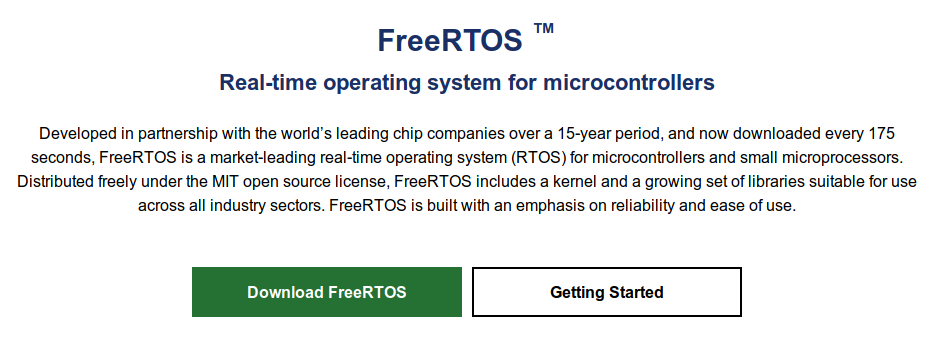
\includegraphics[scale=.5]{images/accueil_site.png}
	\end{center}
\end{figure}

Sur mon affichage aux couleurs inversées, le rose du bouton \enquote{Download
FreeRTOS} est très sexy !\\

Le dépot github indique à ce jour 2774 commits (le dernier il y a 7 jours et 10
contributeurs.
%\\\\
%\enquote{En 2017, le projet et son équipe de \textbf{développeurs} ont été \textbf{acquis par Amazon}}\cite{ref6}.

\subsubsection{Acceptabilité}
\begin{tabular}{lll}
\toprule
	Critère				&	Validé		&	Commentaire	\\
\midrule
	Licence				&	oui			&	historique bancal	\\
	Code source			&	oui			&		\\
	Plateformes cible	&	oui			&	ARM\_CM7	\\
	Communauté			&	oui			&		\\
\bottomrule
\end{tabular}



\subsection{Lepton-rtos}
\subsubsection{Licence}
Mozilla Public License Version 1.1.\\

Incompatible avec la GNU GPL selon gnu.org\cite{ref2} :

{\small
\begin{verbatim}
Il s'agit d'une licence de logiciel libre, pas très stricte en tant que copyleft.
Contrairement à la licence X11 elle présente des restrictions complexes qui la
rendent incompatibles avec la GNU GPL. En effet on ne peut pas, légalement, lier un
module couvert par la GPL et un module couvert par la MPL. C'est pourquoi nous vous
demandons instamment de ne pas utiliser la MPL 1.1.

Cependant, la licence MPL 1.1 permet (article 13) à un programme ou à des portions du
programme d'offrir le choix d'une licence alternative. Si une portion du programme
offre la GNU GPL (ou toute autre licence compatible avec la GPL) comme choix
possible, alors la licence de cette portion du programme est compatible avec la GPL.
\end{verbatim}
}

Ouf ! On a eu chaud, il y a une licence alternative :

{\footnotesize
\begin{verbatim}
Alternatively, the contents of this file may be used under the terms of the eCos GPL license 
(the  [eCos GPL] License), in which case the provisions of [eCos GPL] License are applicable 
instead of those above. If you wish to allow use of your version of this file only under the
terms of the [eCos GPL] License and not to allow others to use your version of this file under 
the MPL, indicate your decision by deleting  the provisions above and replace 
them with the notice and other provisions required by the [eCos GPL] License. 
If you do not delete the provisions above, a recipient may use your version of this file under 
either the MPL or the [eCos GPL] License.
\end{verbatim}
}

Tiens, revoilà le dinosaure !

C'est quand même \enquote{borderline} niveau licence.

\subsubsection{Code source}
Le code source est sur github.com :
\url{https://github.com/lepton-distribution/lepton}.

Dernière modification du code en 2015.

\subsubsection{Plateformes cible}
Simulateur sur PC et ARMs dont :
\enquote{ARM Cortex-M4: STM32F4 Discovery (ST stm32F407)}

\subsubsection{Communauté}
Dernière modification du code en 2015...

Je n'ai pas trouvé de site.

\subsubsection{Acceptabilité}
\begin{tabular}{lll}
\toprule
	Critère				&	Validé		&	Commentaire	\\
\midrule
	Licence				&	oui			&		\\
	Code source			&	oui			&		\\
	Plateformes cible	&	oui			&		\\
	Communauté			&	non			&	Inactif	\\
\bottomrule
\end{tabular}



\subsection{nOS}
\subsubsection{Licence}
Mozilla Public License, version 2.0 mais avec :
\begin{verbatim}
Exhibit B - "Incompatible With Secondary Licenses" Notice

      This Source Code Form is "Incompatible
      With Secondary Licenses", as defined by
      the Mozilla Public License, v. 2.0.
\end{verbatim}

Ce qui la rend incompatible avec la GNU GPL selon gnu.org\cite{ref2}.

\subsubsection{Communauté}
338 commits et 5 contributeurs sur github, dernier commit il y a 22 jours.\\

Pas de site.

\subsubsection{Acceptabilité}
\begin{tabular}{lll}
\toprule
	Critère				&	Validé		&	Commentaire	\\
\midrule
	Licence				&	non			&		\\
	Code source			&	-			&		\\
	Plateformes cible	&	-			&		\\
	Communauté			&	non			&		\\
\bottomrule
\end{tabular}



\subsection{NuttX RTOS}
\subsubsection{Licence}
Licence Apache, version 2.0 : compatible avec la GNU GPL $ \geqslant $ v3.

\subsubsection{Code source}
\url{https://github.com/apache/incubator-nuttx}\\

Le code est rigoureusement organisé, il respecte un \enquote{Coding Standard} très 
détaillé :
\url{https://cwiki.apache.org/confluence/display/NUTTX/Coding+Standard#parmlists}\\

Pas de doxygen.

\subsubsection{Plateformes cible}
{\small
\url{https://github.com/apache/incubator-nuttx/tree/master/boards/arm/stm32f7/nucleo-144}
}
\begin{verbatim}
ST Nucleo F746ZG board from ST Micro is supported.
\end{verbatim}

\subsubsection{Communauté}
Le projet est actif et populaire, github dit 36873 commits et 212 contributors.\\

Le site hébergé par apache se présente sous la forme d'un wiki où on peut trouver
une importante documentation.\\

Il y a également des forums Google Group et LinkedIn.\\

Il y a un petit canal IRC non officiel sur freenode.

\subsubsection{Acceptabilité}
\begin{tabular}{lll}
\toprule
	Critère				&	Validé		&	Commentaire	\\
\midrule
	Licence				&	oui			&		\\
	Code source			&	oui			&		\\
	Plateformes cible	&	oui			&		\\
	Communauté			&	oui			&		\\
\bottomrule
\end{tabular}



\subsection{Prex}
Éteint depuis 2009.

\subsubsection{Acceptabilité}
\begin{tabular}{lll}
\toprule
	Critère				&	Validé		&	Commentaire	\\
\midrule
	Licence				&	-			&		\\
	Code source			&	-			&		\\
	Plateformes cible	&	-			&		\\
	Communauté			&	non			&		\\
\bottomrule
\end{tabular}



\subsection{RIOT OS}
\subsubsection{Licence}
GNU LESSER GENERAL PUBLIC LICENSE Version 2.1.

\subsubsection{Code source}
Le code source est sur github : \url{https://github.com/RIOT-OS/RIOT}.\\

Documenté avec Doxygen.\\

Utilise le \enquote{codingstyle} de linux.


\subsubsection{Plateformes cible}
\url{https://github.com/RIOT-OS/RIOT/tree/master/boards/nucleo-f746zg}

\subsubsection{Communauté}
Le site : \url{https://www.riot-os.org}

La communauté est vaste (28351 commits et 253 contributors sur github) et active.\\

Il y a de la documentation, des mailing lists, un canal IRC sur freenode, l'
\enquote{issue tracker} de github... tout ce qui fait une belle communauté de
développeurs de logiciel libre.

\subsubsection{Acceptabilité}
\begin{tabular}{lll}
\toprule
	Critère				&	Validé		&	Commentaire	\\
\midrule
	Licence				&	oui			&		\\
	Code source			&	oui			&		\\
	Plateformes cible	&	oui			&		\\
	Communauté			&	oui			&		\\
\bottomrule
\end{tabular}



\subsection{RTEMS}
\subsubsection{Licences}
Principalement GNU GPLv2 modifiée :
{\small
\begin{verbatim}
As a special exception, including RTEMS header files in a file, instantiating RTEMS
generics or templates, or linking other files with RTEMS objects to produce an
executable application, does not by itself cause the resulting executable application
to be covered by the GNU General Public License. This exception does not however
invalidate any other reasons why the executable file might be covered by the GNU
Public License.
\end{verbatim}\\
}
Two-Clause BSD license : \enquote{Completely new submissions are encouraged to use
this license.}

\subsubsection{Code source}
Dépot git sur le site : \url{https://git.rtems.org/}.\\

Les commentaires comportent des tags doxygen.\\

Il y a un standard de codage :
\url{https://docs.rtems.org/branches/master/eng/coding.html}.

\subsubsection{Plateformes cible}
Pas précisément le STM32F746ZG mais on peut lire \enquote{STMicroelectronics STM32 F4
and STM32F105} sur la page
\url{https://devel.rtems.org/wiki/TBR/Website/Board\_Support\_Packages}.

\subsubsection{Communauté}
La communauté est active.\\

Le site internet \url{https://www.rtems.org/} comporte 6 pages :
\begin{itemize}
	\item Home ;
	\item Wiki ;
	\item Git ;
	\item Training ;
	\item News Archive ;
	\item Licenses.\\
\end{itemize}

Il y a une boîte \enquote{Community} sur la gauche de la page d'accueil :
\begin{itemize}
	\item Mailing Lists ;
	\item IRC \#rtems (freenode) + logs sur rtems.org ;
	\item Linkedin ;
	\item Twitter ;
	\item Facebook.\\
\end{itemize}

Il est utilisé dans l'industrie spatiale, notamment par les acteurs européens du
domaine selon l'article Wikipédia.

\subsubsection{Acceptabilité}
\begin{tabular}{lll}
\toprule
	Critère				&	Validé		&	Commentaire	\\
\midrule
	Licence				&	oui			&		\\
	Code source			&	oui			&		\\
	Plateformes cible	&	oui			&	STM32F4	\\
	Communauté			&	oui			&		\\
\bottomrule
\end{tabular}



\subsection{SHaRK}
\subsubsection{Licence}
GNU GPLv2.

\subsubsection{Code source}
Dépot SVN (dernière modif en 2008).

\subsubsection{Acceptabilité}
\begin{tabular}{lll}
\toprule
	Critère				&	Validé		&	Commentaire	\\
\midrule
	Licence				&	oui			&		\\
	Code source			&	oui			&		\\
	Plateformes cible	&	-			&		\\
	Communauté			&	non			&	Inactif depuis 2008	\\
\bottomrule
\end{tabular}



\subsection{Trampoline}
\subsubsection{Licence}
GNU GPLv2.\\

Notice de copyright dans le code source :
{\small
\begin{verbatim}
 * Trampoline RTOS
 *
 * Trampoline is copyright (c) CNRS, University of Nantes, Ecole Centrale de Nantes
 * Trampoline is protected by the French intellectual property law.
 *
 * This software is distributed under the GNU Public Licence V2.
 * Check the LICENSE file in the root directory of Trampoline
 *
\end{verbatim}
}

\subsubsection{Code source}
Dépôt github.com : \url{https://github.com/TrampolineRTOS/trampoline}.\\

Tags Doxygen présents dans les commentaires.\\

Le code est un peu bizarre :
\begin{verbatim}
/*
 * MISRA RULE 13 VIOLATION: this function is only used for debug purpose,
 * so production release is not impacted by MISRA rules violated
 * in this function
 */
FUNC(void, OS_CODE) printrl(P2VAR(char, AUTOMATIC, OS_APPL_DATA) msg)
{
\end{verbatim}

Il semble qu'il respecte la norme de programmation MISRA C de la \emph{Motor Industry 
Software Reliability Association} que l'on peu ce procurer pour 45£.\\

Il utilise également le langage de description d'application OIL (Figure 
\ref{fig:oil}).

\begin{figure}[!h]
	\begin{center}
		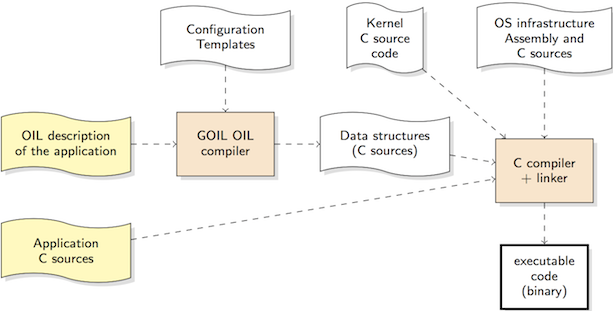
\includegraphics[scale=2.5]{images/trampoline_building.png}
	\end{center}
	\caption[]{\label{fig:oil} The building process of the executable of an
				application using Trampoline \cite{ref7}.}
\end{figure}

\subsubsection{Plateformes cible}
Il a été porté sur STM32F4 Discovery :
\url{https://github.com/TrampolineRTOS/trampoline/wiki/The-STM32F4-Discovery-port}

\subsubsection{Communauté}
Le projet semble entièrement hébergé sur github.com avec actuellement 13
contributeurs. Il y a eu 2682 commits depuis 2006, le dernier date d'il y a 10 jours.
\\

Le wiki contient 16 pages. La page d'accueil donne une description succincte du
projet :
{\small
\begin{verbatim}
Trampoline is a Real Time Operating System (RTOS) which is developed by the Real Time
System Group at LS2N (ex-IRCCyN) Laboratory (France). Trampoline implements the OSEK
and AUTOSAR standards.
\end{verbatim}
}
\subsubsection{Acceptabilité}
\begin{tabular}{lll}
\toprule
	Critère				&	Validé		&	Commentaire	\\
\midrule
	Licence				&	oui			&	+ copyright CNRS	\\
	Code source			&	non			&	MISRA C non libre	\\
	Plateformes cible	&	oui			&	STM32F4	\\
	Communauté			&	non			&	insuffisante	\\
\bottomrule
\end{tabular}



\subsection{Xenomai}
\begin{verbatim}
Xenomai is a Free Software project in which engineers from a wide
background collaborate to build a versatile real-time framework for
the Linux© platform.
\end{verbatim}

À priori nous avions déjà écarté une solution basée sur linux lors d'une discussion
informelle car linux n'est pas un noyau temps réel.\\

Toutefois Xenomai semble y apporter des fonctionnalités de temps réel dur.\\

Bien que linux réponde largement à tous les autre critères technique, je crains que
ça ne soit au prix d'une complexité et d'un poids exagéré du firmware. C'est pourquoi
je l'ai écarté dans un premier temps.\\

Pour moi, il ne fait aucun doute que le STM32F746ZG puisse faire tourner Linux (j'ai 
effectué ma première installation de linux en 1997 sur un 80486@66MHz bien moins
rapide) mais ça nécessiterait d'emblée l'ajout de mémoire externe, le STM32F746ZG ne
disposant que de 320KB de SRAM en interne.

Par exemple on peut lire à propos de uClinux \cite{ref9} :
{\small
\begin{verbatim}
The size of a practical bootable image, with Ethernet, TCP/IP and a reasonable set of
user-space tools and applications confugured, would be in a 1.5 - 2 MBytes ballpark.
With the "two-chips Linux design" concept in mind, a 1.5 MBytes image could possibly
fit into internal Flash of today's Cortex-M microcontrollers. One example of a device
that can hold an image of the size is the STM32F429 Cortex-M4 microcontroller.

Size of external RAM required for run-time Linux operation. The answer we give to our
customers when asked how much RAM is needed is the more the better, but no less than
8 MBytes. Admittedly, it may be possible to run some very basic configurations with
rootfs mounted from NFS or some external device even out of 2 MBytes but frankly this
is more of a joke than a configuration one can build a practical uClinux design on.
\end{verbatim}
}

Pour ceux qui se demande quelle-est la configuration minimale pour un noyau Linux :
\url{http://dmitry.gr/?r=05.Projects&proj=07.%20Linux%20on%208bit} 

\subsubsection{Acceptabilité}
\begin{tabular}{lll}
\toprule
	Critère				&	Validé		&	Commentaire	\\
\midrule
	Licence				&	-			&		\\
	Code source			&	-			&		\\
	Plateformes cible	&	non			&	Linux	\\
	Communauté			&	-			&		\\
\bottomrule
\end{tabular}



\subsection{Erika3}
\subsubsection{Licences}
ERIKA v3 is now distributed under the following three licensing schemes :
\begin{itemize}
	\item GPLv2, with a linking exception allowing the inclusion and linking of
			specific silicon vendor source code (e.g., the register include file, device
			drivers, and so on);
	\item GPLv2 + linking exception license, which will allow a customer to link
			proprietary source code;
	\item Commercial license.
\end{itemize}

\subsubsection{Code source}
Le code est hébergé sur github.com :
\url{https://github.com/evidence/erika3}.\\

Les commentaires comportent des tags Doxygen.\\

On retrouve un peu les mêmes bizarreries que dans le code de Trampoline :
\begin{verbatim}
FUNC(void, OS_CODE) osEE_cortex_m_system_init(void)
{
\end{verbatim}


\subsubsection{Plateformes cible}
Il y a un dossier cortex-m dans erika3/pkg/arch/.


\subsubsection{Communauté}
Le projet semble jeune (environ 2 ans), du moins pour la version 3.\\

Il semble peu actif : dernier commit en septembre 2019.\\

Il y a un wiki et un forum.\\

Le projet semble open-source mais fermé à la contribution.\\

Rien de très excitant en somme.

\subsubsection{Acceptabilité}
\begin{tabular}{lll}
\toprule
	Critère				&	Validé		&	Commentaire	\\
\midrule
	Licence				&	oui			&		\\
	Code source			&	oui			&		\\
	Plateformes cible	&	oui			&	cortex-m	\\
	Communauté			&	non			&	dernier commit en septembre 2019	\\
\bottomrule
\end{tabular}



\subsection{Contiki-ng}
(Suggestion de Clément)
\subsubsection{Licence}
Licence BSD 3 Clauses \cite{ref8}.\\

Cette licence est compatible avec la GNU GPL.

\subsubsection{Code source}
Le code est hébergé sur github : \url{https://github.com/contiki-ng/contiki-ng}\\

Les commentaires comportent des tags doxygen.\\

Il y a un \enquote{Code style} documenté.\\

Le code semble peu commenté mais très lisible.

\subsubsection{Plateformes cible}
Bien qu'il soit avant tout destiné à des SoC de capteurs miniature comme TI CC2538,
il semble supporter l'architecture Cortex-M7 :
\url{https://github.com/contiki-ng/contiki-ng/blob/develop/arch/cpu/arm/cortex-m/CMSIS/core_cm7.h}.

\subsubsection{Communauté}
Le dépot github indique 15345 commits et 193 contributeurs.\\

On y trouve un fichier \enquote{CONTRIBUTING.md} donc il accepte les contributions.\\

Il y a un wiki et un site internet.

\subsubsection{Acceptabilité}
\begin{tabular}{lll}
\toprule
	Critère				&	Validé		&	Commentaire	\\
\midrule
	Licence				&	oui			&		\\
	Code source			&	oui			&		\\
	Plateformes cible	&	oui			&		\\
	Communauté			&	oui			&		\\
\bottomrule
\end{tabular}

Bien qu'il réponde à tous les critères définis à ce stade, je vais l'écarter d'emblée
car ce n'est pas un RTOS : 
\url{https://fr.wikipedia.org/wiki/Contiki#Ex%C3%A9cution_d'applications_en_temps_r%C3%A9el},
\enquote{Contiki n'est pas un système d'exploitation permettant l'exécution
d'applications en temps réel}.



\subsection{Mynewt}
(Suggestion de Clément)
\subsubsection{Licence}
Licence Apache, version 2.0 : compatible avec la GNU GPL $ \geqslant $ v3.\\

Le fichiers LICENSE du dépôt stipule de nombreux fichiers sous d'autres licences,
principalement \enquote{3-clause BSD}, de la ligne 203 à la ligne 685.

\subsubsection{Code source}
Le code source est hébergé sur github : \url{https://github.com/apache/mynewt-core}.\\

À la racine du dépôt on trouve un fichier \enquote{CODING\_STANDARDS.md}.\\

Les commentaires contiennent des tags Doxygen.

\subsubsection{Plateformes cible}
On trouve un dossier \enquote{nucleo-f746zg} dans le dépôt :
\url{https://github.com/apache/mynewt-core/tree/master/hw/bsp/nucleo-f746zg}.

\subsubsection{Communauté}
Le dépôt git indique 9797 commits et 102 contributeurs.\\

Le projet accepte les contributions :
\begin{verbatim}
Contributing

Anybody who works with Apache Mynewt can be a contributing member of the community
that develops and deploys it. The process of releasing an operating system for
microcontrollers is never done: and we welcome your contributions to that effort.
\end{verbatim}

\subsubsection{Acceptabilité}
\begin{tabular}{lll}
\toprule
	Critère				&	Validé		&	Commentaire	\\
\midrule
	Licence				&	oui			&		\\
	Code source			&	oui			&		\\
	Plateformes cible	&	oui			&		\\
	Communauté			&	oui			&		\\
\bottomrule
\end{tabular}



\subsection{Zephyr}
(Suggestion de Clément)
\subsubsection{Licence}
Licence Apache, version 2.0 : compatible avec la GNU GPL $ \geqslant $ v3.

\subsubsection{Code source}
Le code source est hébergé dans un dépôt github :
\url{https://github.com/zephyrproject-rtos/zephyr}.\\

Il respect le \enquote{Linux kernel coding style} et est documenté avec Doxygen.\\

Le dépôt est très copieux et bien organisé.

\subsubsection{Plateformes cible}
La carte nucleo-f746zg est supportée :
\url{https://github.com/zephyrproject-rtos/zephyr/tree/master/boards/arm/nucleo_f746zg}.

\subsubsection{Communauté}
39868 commits, 665 contributeurs, c'est un très gros projet !

\subsubsection{Acceptabilité}
\begin{tabular}{lll}
\toprule
	Critère				&	Validé		&	Commentaire	\\
\midrule
	Licence				&	oui			&		\\
	Code source			&	oui			&		\\
	Plateformes cible	&	oui			&		\\
	Communauté			&	oui			&		\\
\bottomrule
\end{tabular}



\subsection{Résultat de cette première sélection}
7 RTOS répondent aux critères :
\begin{description}
	\item[ChibiOS] \url{http://chibios.org/}
	\item[FreeRTOS] \url{https://www.freertos.org/}
	\item[NuttX] \url{https://nuttx.apache.org/}
	\item[RIOT] \url{https://www.riot-os.org/}
	\item[RTEMS] \url{https://www.rtems.org/}
	\item[Mynewt] \url{https://mynewt.apache.org/}
	\item[Zephyr] \url{https://www.zephyrproject.org/}
\end{description}

\subsection{Autres RTOS}
Au cours de mes recherches je suis tombé sur une autre liste :\\
\url{https://www.osrtos.com/}.\\

Je pensais initialement sortir \enquote{une poignée} c'est a dire 5 RTOS de cette 
présélection afin d'affiner les critères et j'en ai déjà 7. C'est pourquoi je pense
qu'il serait contre-productif d'en ajouter à ce stade.
